% begin module trig-substitutions-ex2
\begin{frame}
\begin{example}[Example 2, p. 504]
\begin{columns}[c]
\column{.4\textwidth}
Find the area enclosed by the ellipse $\frac{x^2}{a^2} + \frac{y^2}{b^2} = 1$.
\begin{itemize}
\item<2->  Let \alert<3-4,7,14,18>{$x = \uncover<4->{3\sin \theta}$}\uncover<4->{, where \alert<10>{$-\pi /2 \leq \theta \leq \pi / 2$}.}
\item<2->  Then \alert<5-6,13>{$\diff x = \uncover<6->{3\cos \theta\diff \theta}$}\uncover<6->{.}
\end{itemize}
\column{.6\textwidth}
\begin{center}
\ \only<-17>{%
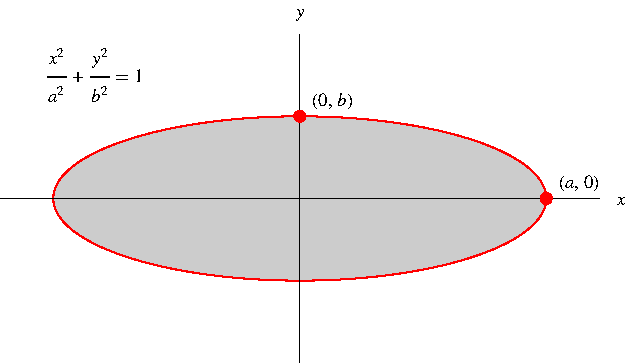
\includegraphics[height=3cm]{trig-substitution/pictures/08-03-ex2a.pdf}%
}%
\only<18->{%
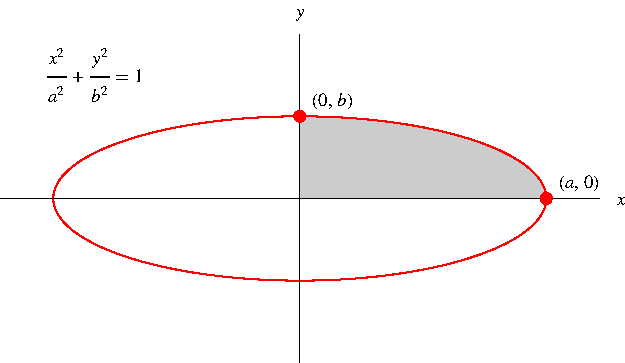
\includegraphics[height=3cm]{trig-substitution/pictures/08-03-ex2b.pdf}%
}%
\end{center}
\end{columns}
\abovedisplayskip=0pt
\belowdisplayskip=0pt
\[
\uncover<2->{%
\alert<12>{%
\sqrt{9 - \alert<7>{x^2}} = 
}%
}%
\uncover<7->{%
\sqrt{9 - \alert<7>{9\sin^2 \theta}} = 
}%
\uncover<8->{%
\sqrt{9 \cos^2 \theta} = 
}%
\uncover<9->{%
3 |\cos  \theta | = 
}%
\uncover<10->{%
\alert<12>{%
3 \cos  \theta  
}%
}%
\]
\abovedisplayskip=0pt
\belowdisplayskip=0pt
\begin{eqnarray*}
\uncover<11->{%
\int \frac{\alert<12>{\sqrt{9-x^2}}}{\alert<14>{x^2}}\alert<13>{\diff x}%
}%
& \uncover<11->{ = } & %
\uncover<11->{%
\int\frac{\alert<12>{3\cos \theta}}{\alert<14>{9\sin^2 \theta}}\alert<13>{3\cos \theta \diff \theta}
}%
\uncover<15->{%
 = \int \cot^2 \theta \diff \theta
}\\%
& \uncover<16->{ = } & %
\uncover<16->{%
 \int (\csc^2 \theta  - 1)\diff \theta
}  \uncover<17->{ = }  \uncover<17->{%
 -\alert<20-21>{\cot \theta} - \theta + C
}\\%
& \uncover<21->{ = } & %
\uncover<21->{%
 -\alert<21>{\frac{\sqrt{9-x^2}}{x}} - \sin^{-1}\left( \frac{x}{3}\right) + C
}%
\end{eqnarray*}
\end{example}
\end{frame}
% end module trig-substitutions-ex2
